\setcounter{section}{0}
\subsection{Exercise 0.1}

For a group $ G $ let $ \set_G $ be the category of sets with a right $ G $ action i.e. 
\begin{itemize}
    \item 
    the objects are tuples $ ( X , \rho_X ) $ where $ X $ is a set and $ \rho \colon X \times G \to X $ is a map satisfying for all $ g , h \in G $ and $ x \in X $ that $ \rho_X ( x , g h ) = \rho_X ( \rho_X ( x , g ) , h ) $ and furthermore $ \id_X = \rho_X ( - , e ) $ for $ e $ the neutral element of $ G $, and
    \item 
    a morphism $ \phi \colon ( X , \rho_X ) \to ( Y , \rho_Y ) $ is given by a map $ \phi \colon X \to Y $ satisfying $ \phi \circ \rho_X = \rho_Y \circ ( \phi \times \id_G ) $ .
\end{itemize}
Recall that we view $ G $ as a category $ B G $ with one object $ \star $ and  $ \Hom_{ B G } ( \star, \star ) = G $. 
Show that there is and isomorphism of categories between $ \set_G $ and $ \widehat{ BG } $, the category of presheaves over $ B G $.

\subsection{ Exercise 0.2 }

For a set $ Y $, show that there is an isomorphism of functors $ \set^{ \op } \times \set \to \set $
\[
    \Hom_{ \set } ( - \times Y , ? ) \cong  \Hom_{ \Set } ( - , \Hom_{ \set } ( Y , ? ) ).
\]

\subsection{ Exercise 0.3 }

Let $ \eta \colon F \to G $ be a natural transformation of two functors $ F , G \colon \mathcal{ A } \to \mathcal{ B } $.
Show that $ \eta $ is a natural isomorphism, i.e. there exists a natural transformation $ \eta' \colon G \to F $ such that $ \eta' \circ \eta = \id_F $ and $ \eta \circ \eta' = \id_G $, if and only if for every $ a \in \mathcal{ A } $ the morphism $ \eta_a \colon F ( a ) \to G ( a ) $ is an isomorphism.

\subsection{ Exercise 0.4 }

Fix an object $ x \in \mathcal{ C } $ of a category $ \mathcal{ C } $. 
The slice category $ \mathcal{ C } / x $ of $ \mathcal{ C } $ over $ x $ is defined as follows.
\begin{itemize}
    \item 
    The objects are tuples $ ( a , \pi ) $ with $ a  \in \mathcal{ C } $ an object and a morphism $ \pi \colon a \to x $. 
    \item 
    A morphism $ f \colon ( a , \pi ) \to ( b , \rho ) $ is given by a morphism $ f \colon a \to b $ such that $ \pi = \rho \circ f $.
\end{itemize}

After convincing yourself that this defines a category, do the following.

\begin{enumerate}[label=(\alph*)]

    \item 
    Show that there exists a final object in $ \mathcal{ C } / x $, i.e. an object $ ( e , \rho ) $ such that for any object $ ( a , \pi ) $ there is a unique morphism $ f \colon ( a , \pi ) \to ( e , \rho ) $.
    \item 
    
    Define the coslice category $ x / \mathcal{ C } $ of elements under $ x $.
    
    \item 
    Describe $ ( \mathcal{ C } / x )^{ \op } $ as a slice or coslice category.
    
\end{enumerate}

\section{ Sheet 1 }

\subsection{ Exercise 1.1 }

Alice and Bob are randomly placed in a $ 3 \times 2 $-grid on two different squares.
\begin{center}
    \begin{tikzpicture}
        \draw (-3,2) -- (3,2);
        \draw (-3,-2) -- (3,-2);
        \draw (-3,0) -- (3,0);
        \draw (-3,-2) -- (-3,2);
        \draw (-1,-2) -- (-1,2);
        \draw (1,-2) -- (1,2);
        \draw (3,-2) -- (3,2);
        \node[red, scale = 2] (B) at (2,1) {B};
        \node[blue, scale = 2] (A) at (-2,-1) {A};
    \end{tikzpicture}
\end{center}

Every turn they are moving to an orthogonally adjacent square which is not currently occupied and they never move to the same square.

\begin{enumerate}[label=(\alph*)]

    \item 
    Describe the groupoid of configurations by connecting two configurations if they are connected by a single turn.  
    
    \item 
    Which of the following configurations can be reached from the above? 
    How many connected components does the groupoid have?
    \begin{center}
        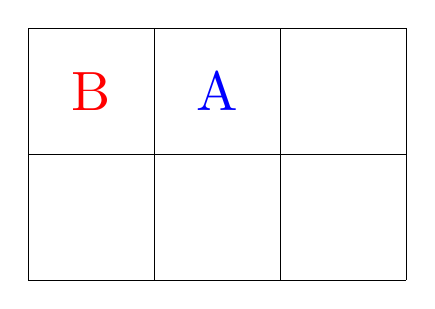
\begin{tikzpicture}[scale = 0.8]
            \draw (-3,2) -- (3,2);
            \draw (-3,-2) -- (3,-2);
            \draw (-3,0) -- (3,0);
            \draw (-3,-2) -- (-3,2);
            \draw (-1,-2) -- (-1,2);
            \draw (1,-2) -- (1,2);
            \draw (3,-2) -- (3,2);
            \node[red, scale = 2] (B) at (-2,1) {B};
            \node[blue, scale = 2] (A) at (0,1) {A};
        \end{tikzpicture}
        \qquad
        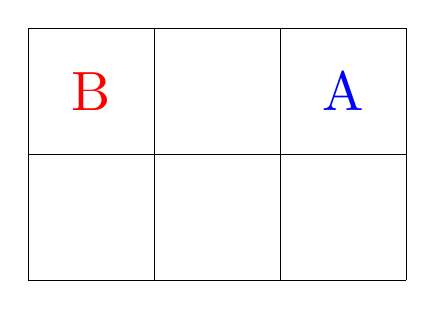
\begin{tikzpicture}[scale = 0.8]
            \draw (-3,2) -- (3,2);
            \draw (-3,-2) -- (3,-2);
            \draw (-3,0) -- (3,0);
            \draw (-3,-2) -- (-3,2);
            \draw (-1,-2) -- (-1,2);
            \draw (1,-2) -- (1,2);
            \draw (3,-2) -- (3,2);
            \node[red, scale = 2] (B) at (-2,1) {B};
            \node[blue, scale = 2] (A) at (2,1) {A};
        \end{tikzpicture}
    \end{center}

    \item 

    Describe what additional information the groupoid holds over the equivalence classes of configurations up to moves.
    
\end{enumerate}

\subsection{ Exercise 1.2 ( linear Yoneda Lemma 1) }

For an (associative and unital) ring $ R $ let $ B R $ be the category associated to the multiplicative monoid of $ R $.
Show that there is an isomorphism of categories $ \psi \colon \Mod_R \to \Fun_{ \mathbb{ Z } } ( ( B R )^{ \op } , \Ab ) $ relating the category of right $ R $-modules into the category of '$ \mathbb{ Z } $-linear presheaves over $ B M $', i.e. contravariant $ \mathbb{ Z } $-linear functors from $ B R $ to the category of abelian groups $ \Ab $.

\subsection{ Exercise 1.3 ( linear Yoneda Lemma 2 )}

Let $ R $ be a ring and let $ \prescript{  }{ R }{ R }_R$ be $ R $ viewed as an $ R $-$ R $-bimodule.

\begin{enumerate}[label=(\alph*)]

    \item 
    Show that for any $ R $-$ R $-bimodule $ N $ and any $ M \in \mod_R $ that $ \Hom_{ \mod R } ( N , M ) $ carries the structure of a right $ R $-module via $ ( f r ) ( x ) \coloneqq f ( r x ) $. 
    Deduce that $ N $ induces a functor
    \[
        \Hom_{\mod R } ( N , - ) \colon \mod R \to \mod R.
    \]
    
    \item 
    
    Show that there is an isomorphism of functors $ \Hom_{ \mod R } ( \prescript{}{ R }{ R }_R , - ) \cong \id_{ \mod R } $ given by evaluation at $ 1 \in R $.
\end{enumerate}

\subsection{ Exercise 1.4 (pullbacks in $\set$) }

Consider four sets $ A , B , C $ and $ E $ and assume that $ A , B \subseteq C $ with the inclusions $ \iota_A $ and $ \iota_B $.

\begin{enumerate}[label=(\alph*)]
    \item 
    Show that for any two maps $ \phi_A \colon E \to A $ and $ \phi_B \colon E  \to B $ such that $ \iota_A \circ \phi_A = \iota_B \circ \phi_B $ there is a unique map $ \phi \colon E \to A \cap B $ such that $ \phi_A = i_A \circ \phi $ and $ \phi_B = i_B \circ \phi $ for $ i_A $ and $ i_B $ the respective inclusions of $ A \cap B $. 
    \[
    \begin{tikzcd}
        E 
        \ar[rd, dashed, " \exists ! \phi" ]
        \ar[rrd, bend left, " \phi_A" ]
        \ar[rdd, bend right, " \phi_B" ']
        \\
        &
        A \cap B
        \ar[r , " i_A " ]
        \ar[d , " i_B " ]
        &
        A
        \ar[ d , " \iota_A" ]
        \\
        &
        B
        \ar[r, " \iota_B " ]
        &
        C
    \end{tikzcd}
    \]

    \item 
    Give an example of two maps $ f_A \colon A \to D $ and $ f_B \colon B \to D $ such that $ A \cap B $ does not have the above property for $ f_A $ and $ f_B $ instead of $ \iota_A $ and $ \iota_B $.

    \item 
    Show that in this more genral setting that
    \[
        A \times_D B \coloneqq \{ ( a, b ) \in A \times B \mid f_A ( a ) = f_B ( b ) \}
    \]
    with the canonical projections $ p_A, p_B$ satisfying the universal property from before.
    \[
    \begin{tikzcd}
        E 
        \ar[rd, dashed, " \exists ! \phi" ]
        \ar[rrd, bend left, " \phi_A" ]
        \ar[rdd, bend right, " \phi_B" ']
        \\
        &
        A \times_D B
        \ar[r , " p_A " ]
        \ar[d , " p_B " ]
        &
        A
        \ar[ d , " f_A" ]
        \\
        &
        B
        \ar[r, " f_B " ]
        &
        D
    \end{tikzcd}
    \]

    \item 
    What is the relation between $ A \cap B $ and $ A \times_C B$ for part (a) ?
\end{enumerate}


\section{Sheet 2}

\subsection{Exercise 2.1}

Show that two objects $ a , b \in A $ in a category $ A $ are isomorphic if and only if their respresentable presheaves $ \Hom_A ( - , a ) $ and $ \Hom_A ( -, b ) $ are isomorphic in $ \widehat{ A } $.

\subsection{Exercise 2.2}

Consider a functor $ F \colon A  \to \mathcal{ C } $ from a small category $A$.

\begin{enumerate}
    \item 
    Show that if $ A $ is an initial object $ \emptyset $, then the limit of $ F $ exists.

    \item 
    Show that if $ A $ has a final object $ e $, then the colimit of $ F $ exists.
\end{enumerate}

\subsection{Exercise 2.3}{ (limits and equalizers)}

Let $ F \colon A \to \set $ be a functor from a small category to the category of sets.
Recall that we have shown in the lecture that the limit of $ F $ exists and is given by 
\[
    \lim_A F \coloneqq \bigg\{ x \in \prod_{ a \in A } F ( a ) \mid \forall u \colon a \to b \quad F ( u ) ( x_a ) = x_b \bigg\}
\]
together with the canonical projections.

\begin{enumerate}[label=(\alph*)]
    \item 
    Show that the inclusion $ \lim_A F \subseteq \prod_{ a \in A } F ( a ) $ exhibits $ \lim_A F $ as the equalizer (= limit of the following diagram)
    \[
    \begin{tikzcd}
        \prod_{ a \in A } F ( a ) 
        \ar[r , shift left, " \phi "]
        \ar[r , shift right, " \psi "']
        &
        \prod_{ \substack{ u \colon s \to t \\ \text{ in } A} } F ( t )
    \end{tikzcd}
    \]
    where $ \phi ( x )_u = F ( u ) ( x_{ s ( u ) } ) $ and $ \psi ( x )_u = x_{ t ( u ) }$.

    \item 
    Let $ \coprod $ denote the disjoint union of sets. 
    Assume that the coequalizer ( = colimit of the following diagram ) 
    \[
    \begin{tikzcd}
        \coprod_{ \substack{ u \colon s \to t \\ \text{ in } A} } F ( t )
        \ar[r , shift left, " \phi "]
        \ar[r , shift right, " \psi "']
        &
        \coprod_{ a \in A } F ( a ) 
    \end{tikzcd}    
    \]
    exists where for $ y \in F ( s ( v ) ) \subseteq \coprod_{ \substack{ u \colon s \to t \\ \text{ in } A} } F ( t ) $ we have $ \phi ( y ) = F ( v ) ( y ) \in F ( t ( v ) ) \subseteq \coprod_{ a \in A } F ( a ) $ and $ \psi ( y ) = y \in F ( s ( v ) ) \subseteq \coprod_{ a \in A } F ( a ) $. Show that it is a colimit of $ F $ with the canonical maps fro $ F ( a ) $.
\end{enumerate}

\subsection{ Exercise 2.4 (colimits in Set) }
\begin{enumerate}[label=(\alph*)]
    \item 
    Show that the disjoint union of sets defines a coproduct in the category of sets, i.e. show that for every family of sets $ ( U_i )_{ i \in I } $ their disjoint union $\coprod_{ i \in I } U_i $ together with the canonical inclusion $ U_j \subseteq \coprod_{ i \in I } U_i $ is the colimit of the functor $ U \colon I \to \Set $ assigning to each $ i \in I $ the set $ U_i $.
    Here $ I $ is some indexing set.

    \item 
    Show that any coequalizer (= colimit of the following diagram ) 
    \[
    \begin{tikzcd}
        U 
        \ar[r, shift left, " \phi "]
        \ar[r, shift right, " \psi "']
        & 
        V
    \end{tikzcd}
    \]
    exists in Set by considering the smallest equivalence relation on $ V $ such that $ v \sim v' $ whenever there is some $ u \in U $ such that $ \phi ( u ) $ and $ \psi ( u ) = v' $.

    \item 
    Conclude using Exercise 2.3 that Set is cocomplete, i.e. every small colimit exists.
\end{enumerate}

\section{ Exercise 3.1 }

Consider two small categories $ A $ and $ B $ and a functor $ F \colon B \to \Fun ( A , \mathcal{ C } ) $. Assume further that $ \lim_B ( \ev_a \circ F ) $ exists in $ \mathcal{ C } $ for every $ a \in A $.

\begin{enumerate}[label=(\alph*)]
    \item 
    Show that a cone $ C $ of $ F $ is a limit cone if and only if for every $ a \in A $
    the evaluation $  C ( a ) $ is a limit cone of $ \ev_a \circ F $.

    \item 
    Deduce that for any small category $ A $ the category of presheaves $ \widehat{ A } $ is complete and cocomplete.

    \item 
    [Bonus] 
    We aim to show that the converse of the above is not true in general, i.e if not all
    $ \lim_B ( \ev_a \circ F ) $ exists, then $ \lim_B F $ might still exist ( and consequentially $( \lim_B F ) ( a ) $ is not a limit cone of $ \ev_a \circ F $ for some $ a \in A $.

    For this we will reformulate the property of a morphism being a monomorphism in terms of a pullback and show that there might exist monomorphisms in $ \Fun ( A , \mathcal{ C } )$ which are not pointwise monomorphisms. Fix $ A  \coloneqq \{ 0 < 1 \} $ to be the category with two objects and one morphism between them.
    Then $ \Fun ( A , \mathcal{ C } ) $ is the morphism category in $ \mathcal{ C } $.
    We now take $ \mathcal{ C } $ to be the category which does contain a non-monomorphism, explicitely let $ \mathcal{ C }$ be given by
    \[
    \begin{tikzcd}
        x 
        \ar[r, bend left, "f"]
        \ar[r, bend right, "g"']
        &
        y
        \ar[r, "h"]
        &
        z
    \end{tikzcd}
    \]
    with the relation $ h \circ f = h \circ g$.
    \begin{itemize}
        \item 
        Show that a morphism $ u \colon s \to t $ in a category is a monomorphism if and only if 
        \[
        \begin{tikzcd}
            s 
            \ar[d, "\id_s"]
            \ar[r, "\id_s"]
            &
            s
            \ar[d, "u"]
            \\
            s 
            \ar[r, "u"]
            & 
            u
        \end{tikzcd}
        \]
        is a pullback diagram.

        \item 
        Show that there is a monomorphism $ u \colon f \to h $ in $\Fun ( A , \mathcal{C} )$ such that $ u_1 $ is not a monomorphism.

        \item 
        Describe a $ B $ and a functor $ F  \colon B \to \Fun ( A , \mathcal{C} ) $ giving the desired counterexample.
        
    \end{itemize}
\end{enumerate}

\subsection{ Exercise 3.2 }

Let $ F \colon A \to \mathcal{ C } $ be a functor from a small category. Let $ \Tilde{ F } \colon A \to  \mathcal{ C } \to \widehat{ \mathcal{ C } } $ be the composition of $ F $ with the Yoneda embedding $ \mathcal{ C } \to \widehat{ \mathcal{ C } } $. Recall from Exercise 3.1 that the limit $ \lim_A \Tilde{ F } $ exists.

\begin{enumerate}[label=(\alph*)]
    \item 
    Show that there is a bijection between representations of $\lim_a \Tilde{ F } $ and limit cones of $ F $.

    \item 
    Deduce that the limit of $ F $ exists if and only if $ \lim_A \Tilde{ F } $ is representable, i.e. there exists some $ c_F \in \mathcal{ C } $ such that $ \lim_A  \Tilde{ F } \cong \Hom_{ \mathcal{ C } } ( - , c_F ) . $ 

    \item 
    Conclude that the Yoneda embedding $ \mathcal{ C } \to \widehat{ \mathcal{ C } } $ preserves limits.
\end{enumerate}

\subsection{Exercise 3.3}

Show that the inclusion $ \iota \colon \Gpd \to \Cat $ of small groupoids into the category of small categories has a right adjoint given by "forgetting" all non-isomorphisms in a given category.

\subsection{Exercise 3.4}

Let $ L \dashv R $ be an adjoint pair of functors where $ L \colon \mathcal{ C } \to \mathcal{ D } $.
Recall that we define unit $ \eta \colon \id_{ \mathcal{ C } } \to R \circ L $ the image of $ \id_{ L ( c ) } $ under the adjunction isomorphism
\[
    \phi_{ ( c , L ( c ) ) } \colon \Hom_{\mathcal{ D } } ( L ( c ) , L ( c ) ) \cong \Hom_{ \mathcal{ C } }( c, R ( L ( c ) ) )
\]
for every $ c \in \mathcal{ C } $ and the counit $ \epsilon \colon L \circ R \to \id_{ \mathcal D } $ as the image of $ \id_{ R ( d ) } $ under the adjunction isomorphism
\[
    \phi^{ -1 }_{ ( R ( d ) , d ) } \colon \Hom_{ \mathcal{ C } } ( R ( d ) , R ( d ) ) \cong  \Hom_{ \mathcal{ D } }( L ( R ( d ) ) , d ) 
\]
for every $ d \in \mathcal{ D } $. 
Show the following 
\begin{enumerate}
    \item 
    The assignment $ \epsilon $ is indeed a natural transformation.

    \item 
    Without using $ L \dashv R $, show that $ \Tilde{ \phi }_{ ( c ,d ) } \coloneqq \eta_c^* \circ R_{ L ( c ) , d } $ defines a natural transformation
    \[
        \Tilde{ \phi } \colon \Hom_{ \mathcal{ D } }( L ( - ) , ?  ) \to \Hom_{ \mathcal{ C } } ( - , R ( ? ) ). 
    \]

    \item 
    There is an adjunction $ R^{ \op } \dashv L^{ \op } $ between the opposite categories with uni $ \epsilon^{ \op } \colon \id_{ \mathcal{ D }^{ \op } } \to L^{ \op } \circ R^{ \op } $ and counit $ \eta^{ \op } \colon R^{ \op } \circ L^{ \op } \to \id_{ \mathcal{ C  }^{\op} } $.

    \item 
    For any $ d \in \mathcal{ D } $ the category $ L / d $ has the final object $ ( R ( d ) , \epsilon_d \colon L R ( d ) \to d ) $.

    \item 
    Given a second adjunction $ L' \dashv R' $ with $ L' \colon \mathcal{ D} \to \mathcal{ A } $ and a unit $ \eta' $ and counit $ \epsilon' $, the counit of the composed adjunction $ L' \circ L \dashv R  \circ R' $ is given by $ \epsilon'_{ ( - ) } \circ L' ( \epsilon_{ R' ( - ) } ) $.

    \item 
    Any right adjoint $ R' $ of $ L , L \dashv R' $, is isomorphic to $ R $.
\end{enumerate}

\section{Exercise sheet 4}

\subsection{Exercise 4.1}
Let $ L \colon \mathcal{ C } \to \mathcal{ D } $ be a functor between small categories.

\begin{enumerate}[label=(\alph*)]
    \item 
    For $ d \in \mathcal{ D } $ describe the category of elements of the presheaf $\Hom_{\mathcal{ D } } ( L ( - ) , d ) \in \widehat{ \mathcal{ C } }$.

    \item 
    Show that $ L $ admits a right adjoint if and only if for every $d \in \mathcal{ D } $ the category of elements $ \int^{ \mathcal{ C } } \Hom_{ \mathcal{ D } } ( L ( - ) , d ) $ admits a final object.
\end{enumerate}

\subsection{Exercise 4.2}
Let $ A $ be a small category and $ a \in A $ some object.

\begin{enumerate}[label=(\alph*)]
    \item 
    Show that $ \Hom_{\widehat{A}}( \widehat{a} , - ) \colon \widehat{A} \to \Set $ preserves colimits, i.e. for any functor $ F \colon I \to \widehat{ A } $ the canonical map 
    \[
        \colim_I ( \Hom_{ \widehat{ A } } ( \widehat{ a } , - ) \circ F ) \to \Hom_{ \widehat{ A } }( \widehat{ a }, \colim_I F )
    \]
    is an isomorphism.

    \item 
    Deduce that $\Hom_{\widehat{A}} ( \widehat{a} , - ) $ admits a right adjoint and describe it.
\end{enumerate}

\subsection{4.3}
Let $ u \colon A \to  B $ be a functor between small categories. 
Let $ u* \colon \widehat{ B } \to \widehat{ A } $ denote the functor obtained by precomposition with $ u $.

\begin{enumerate}[label=(\alph*)]
    \item 
    Show that $u^*$ preserves colimits.

    \item 
    Deduce that there exists a right adjoint $ u^* \dashv u_* $.

    \item 
    Give an explicit description of $ u _*$.

    \item 
    Confirm directly that $ u^* \dashv u_* $ by giving the adjunction isomorphism explicitly.
\end{enumerate}

\subsection{Exercise 4.4}

Let $ X $ be a presheaf over a small category $ A $. Recall from the lecture the canonical functor.
\[
    u \colon \int^A X \to \widehat{ A } / X 
\]
sending $ ( a , s \in X_a ) $ to $ s \colon \widehat{ a } \to X $, where $ \int^A X $ is the category of elements of $ X $. 
Hence, by extending by colimits we obtain a functor
\[
    u_! \colon \widehat{\int^A X} \to \widehat{A} / X
\]
which we aim to show is equivalence, most of which was done in the lecture. 
Show the remaining claims.

\begin{enumerate}[label=(\alph*)]
    \item 
    The slice category $ \widehat{A} / X $ is cocomplete.

    \item 
    For any $ ( a , s \colon a \to X ) \in \int^A X $ the functor $ \Hom_{\widehat{A}/X} ( u_! ( \widehat{ ( a ,s )} ) , - ) $ preserves colimits.

    \item 
    Any $ ( Y , f \colon Y \to X ) $ can be obtained as a colimit of a diagram in the essential image of $ u $.
\end{enumerate}

\section{ Exercise Sheet 5 }

\subsection{ Exercise 5.1}

Let $ \mathcal{ C } $ and $ \mathcal{ D } $ be two cocomplete categories where $ \mathcal{ C } $ is small and let $  D \colon I \to \mathcal{ C } $ be a diagram in $ \mathcal{ C } $.

\begin{enumerate}[label=(\alph*)]
    \item 
    Show that there is a natural transformation of functors $ \Fun ( \mathcal{ C }, \mathcal{ D } \to \mathcal{ D } $
    \[
        can \colon \colim_I D^* ( - ) \to \ev_{ \colim_I D}.
    \]
    
    \item 
    Deduce that if $ F $ and $ G $ are two isomorphic funtors in $ \Fun ( \mathcal{ C } , \mathcal{ D } ) $, then $ F $ is colimit preserving if and only if $ G $ is.
\end{enumerate}

\subsection{ Exercise 5.2}

Consider an adjunction $ L \dashv R $ where $ L \colon \mathcal{ C } \to \mathcal{ D } $.

\begin{enumerate}[label=(\alph*)]

    \item 
    Show that for a $ d \in \mathcal{ D } $ the counit $ \epsilon_d $ at $ d $ is an isomorphism if and only if $ R $ induces a natural isomorphism 
    \[
        R_{d,-}\colon \Hom_{\mathcal{ D } } ( d, - ) \to \Hom_{ \mathcal{ C } } ( R ( d ) , R ( - ) ). 
    \]

    \item 
    Deduce that $ R $ is fully faithful if and only if the counit $ \epsilon \colon L \circ R  \to \id_{\mathcal{ D } } $ is an isomorphism.

    \item 
    Give the dual statement to (b) and give a proof reducing the statement to (b).

    \item 
    Show that if $ R $ is fully faithful, then $ c \in \mathcal{ C } $ is in the essential image of $ R $ if and only if the unit morphism $ \eta_c $ is an isomorphism at $ c $.
    
\end{enumerate}

\subsection{ Exercise 5.3 }

Let $ u \colon A \to B $ be a functor between small categories.
Recall from the lecture and Exercise 4.3 that we have a triple of adjunctions $ u_! \dashv u^* \dashv u_* $ where $ u^* \colon  \widehat{ B } \to \widehat{ A } $. 
Assume further that $ u $ is fully faithful.

\begin{enumerate}[label=(\alph*)]

    \item 
    Show that $ u_* $ is fully faithful. 

    \item   
    Show that $ u_! $ is fully faithful.
    \newline
    (Hint: Show that the class $ \{ X \in \widehat{ A } \mid \eta_X \text{ is invertible } \} $ is closed under colimits and contains all representable presheaves.)
    
\end{enumerate}

\subsection{ Exercise 5.4 }

Show that the functor $ \widehat{ \Delta }  \to \SetD $ which remembers only the face and degeneracy maps and is the identity on morphisms is an isomorphism of categories. 
In particular,
 \begin{itemize}
     \item 
     show that the functor is well defined by showing that the co-face and co-degeneracy maps satisfy the cosimplicial identities.
     \begin{align*}
         d^jd^i &= d^i d^{j-1} \quad \text{ if } i < j
         \\
         s^j s^i &= s^i s^{j+1} \quad \text{ if } i \leq j
     \end{align*}
     \qquad
     $
     s^j d^i=
     \begin{cases}
         d^i s^{j-1} &\text{ if } i < j 
         \\
         \id &\text{ if } i \in \{ j , j + 1 \}
         \\
         d^{i-1} s^j &\text{ if } i > j = 1
     \end{cases}
     $
     Recall that the co-face maps $ d^i \coloneqq d_n^i $ and co-degeneracy maps $ s^i \coloneqq s_n^i $ are defined as follows for each $ n \in \mathbb{ N }_+ $ respective $ n \in \mathbb{ N }_0 $ and $ 0 \leq i \leq n $.  
     \begin{align*}
         d^i = d_n^i \colon [ n - 1 ] &\to [ n ]
         \\
         k &\mapsto 
         \begin{cases}
             k & \text{ if } k < i 
             \\
             k+1 & \text{ if } i \leq k 
         \end{cases}
     \end{align*}
     \quad
     \begin{align*}
         s^i = s_n^i \colon [ n n 1 ] &\to [ n ]
         \\
         k &\mapsto 
         \begin{cases}
             k & \text{ if } k \leq i 
             \\
             k-1 & \text{ if } i < k 
         \end{cases}
     \end{align*}

     \item  
     For the inverse, show that a morphism $ \sigma \colon [m] \to [n] $ in $ \Delta $ can be uniquely written as
    \[
        \sigma 
        =
        d_n^i_s
        \circ d_{ n - 1 }^{i_{s-1}} 
        \circ 
        \dotsm 
        \circ
        d_{ n - s + 1 }^{i_1}
        \circ
        s_{ m - t }^{j_1}
        \circ 
        \dotsm
        \circ
        s_{ m - 2 }^{ j_{t-1}}
        \circ 
        s_{ m - 1 }^j_t
    \]
    with $ 0 \leq i_1 < i_2 < \dotsm < i_s \leq n $ and $ 0 \leq j_1 < j_2 < \dotsm < j_t < m $ and $ n-s = m-t $.
\end{itemize}

\section{ Exercise sheet 6 }

\subsection{ Exercise 6.1 }

Fix $ n \in \mathbb{ N }_+ $.
Define the simplicial subset $ \partial \Delta^n \subseteq \Delta^n $ by
\[
    \partial \Delta^n ( [ m ] ) \coloneqq \{ \sigma \colon [ m ] \to [ n ] \text{ non-surjective } \}
\]
and similarly, define for $ 0 \leq k \leq n $ the simplicial subset $ \Lambda_k^n \subseteq \partial \Delta^n $ by
\[
    \Lambda_k^n( [ m ] ) \coloneqq \{ \sigma  \in \partial \Delta^n ( [ m ] ) \mid \sigma ( [ m ] ) \neq [ n ] \setminus \{ k \} \}.
\]
\begin{enumerate}[label=(\alph*)]
    
    \item 
    Confirm that the above are indeed simplicial subsets.

    \item 
    Show one of the following 
    \begin{itemize}
    
        \item 
        $ \partial \Delta $ is the smallest simplicial subset of $ \Delta^n $ such that $ \{ d_n^i \mid 0 \leq i \leq n \} \subseteq \partial \Delta^n ( [ n - 1 ] ) $.

        \item 
        $\Lambda_k^n$ is the smallest simplicial subset of $ \Delta^n $ such that $ \{ d_n^i \mid 0 \leq i \leq n \wedge i \neq k \} \subseteq \Lambda^n_k ( [ n - 1 ] )$.
        
    \end{itemize}

Recall that we may view $ \Delta $ as a category of posets, so that we may compute the nerve of ( subsets of ) $ [ n ] $ as partially ordered set.
Moreover, we may associate to $ [ n ] $ the category $ \Sub_* ( [ n ] ) $ of non-empty proper full subcategories, i. e. $ [ n ] \notin \Sub_* ( [ n ] ) $, and morphisms given by inclusions.
Similarly, we define for $ k \in [ n ] $ the full subcategory $ \Sub_*^k ( [ n ] ) \coloneqq \{ k \in E \in \Sub_* ( [ n ] ) \subseteq  \Sub_* ( [ n ] )$.

    \item 
    Show one of the following.

    \begin{enumerate}
        \item 
        \[
            \partial \Delta^n
            \cong 
            \bigcup_{ E \in \Sub_* ( [ n ] ) } N ( E ) \coloneqq 
            \colim_{ E \in \Sub_* ( [ n ] ) } N ( E ) 
        \]

        \item 
        \[
            \partial \Delta^n
            \cong
            \bigcup_{ E \in \Sub_* ( [ n ] ) } N ( E ) \coloneqq 
            \colim_{ E \in \Sub_* ( [ n ] ) } N ( E ) 
        \]
    \end{enumerate}

    \item 
    Justify the notation $ \bigcup $.
    
\end{enumerate}

\subsection{ Exercise 6.2 }

Let $ \Delta_{ \leq n } $ be the full subcategory of $ \Delta $ of the elements $ [ 0 ] , [ 1 ] , \dotsc , [ n ] $.
The inclusion $ \iota_n \colon \Delta_ { \leq n } \to \Delta $ induces a truncation functor $ \tr_n \coloneqq ( \iota_n )^* \colon \Set_{ \Delta } \to \widehat{ \Delta_ { \leq n } } $.

\begin{enumerate}[label=(\alph*)]
    
    \item 
    Show that $ \tr_n $ admits both a left and a right adjoint, $ \sk_n \dashv \tr_n \dashv \cosk_n $, which are both fully faithful.

    \item 
    Deduce that we have an adjunction $ \bold{sk_n} \coloneqq \sk_n \circ \tru_n \dashv \cosk_n \circ\tru_n \eqqcolon \bold{ cosk_n } $ of endofunctors of $ \SetD $.
    
\end{enumerate}

The essential image of $ \sk_n $ are called the $ n $-skeletal simplicies while the essential image of $ \bold { cosk_n } $ are the $ n $-coskeletal simplices.

\begin{enumerate}[label=(\alph*), resume]
    \item 
    Show that a simplicial set $ X $ is $ n $-skeletal if and only if 
    
    $ \tru_n \colon \Hom_{ \SetD } ( X , - ) \to \Hom_{ \widehat{ \Delta{ \leq n }}} ( \tru_n X , \tru_n ( - ) ) $ is an isomorphism of functors.

    \item 
    Show that a simplicial set $ Y $ is $ n $-coskeletal if and only if
    
    $ \tru_n \colon \Hom_{ \Set_\Delta } ( - , Y ) \to \Hom_{ \widehat{ \Delta_{ \leq n }} } ( \tru_n ( - ) , \tru_n Y ) $ is an isomorphism of functors.
\end{enumerate}

\subsection{ Exercise 6.3 }

\begin{enumerate}[label=(\alph*)]
     
     \item 
     Show that a map $ F \colon X  \to N ( \mathcal{ C } ) $ to the nerve of a category $ \mathcal{ C } $, is completely determined by a map $ u \colon X_1 \to \Mor ( \mathcal{ C } ) $ such that 
     \begin{enumerate}
         \item 
         for all $ x \in X_0 $ we have that $ u ( s_0 ( x ) ) $ is an identity and 

         \item 
         for any $2$-simplex $ \sigma \in X_2 $ we have that $ u ( d_1 ( \sigma ) ) = u ( d_0 ( \sigma ) ) \circ u ( d_2 ( \sigma ) )$.
     \end{enumerate}

     \item 
     Deduce that the nerve of a category is 2-coskeletal.

     \item 
     Conclude that the nerve $ N \colon \Cat \to \SetD $ is fully faithful.
     
\end{enumerate}

\subsection{ Exercise 6.4 }

Consider the functor $ \Op \colon \Delta \to \Delta $ which is the identity on objects and for $ \sigma : [ n ] \to [ m ] $
\[
    \Op ( \sigma ) ( i ) 
    \coloneqq
    m - \sigma ( n - i )
\]
Let $ ( - )^{ \op } \coloneqq \Op^* \colon \SetD \to \SetD $ be the corresponding involution of the category of simplicial sets.

\begin{enumerate}[label=(\alph*)]
    \item 
    Show that $ \Op $ is a well defined involution.

    \item 
    For a simplicial set $ X $, describe the face and degeneracy maps of $ X ^{ \op } $.

    \item 
    Show that for a category $ \mathcal{ C } $ we have an isomorphism $ N ( \mathcal{ C }^{\op} ) \cong N ( \mathcal{ C } )^{\op} $.

    \item   
    Show that for a topological space there is an isomorphism $ \Sing ( X ) \cong \Sing ( X )^{ \op } $ for the singular complex of $ X $.
\end{enumerate}

\section{Exercise Sheet 7}

\subsection{Exercise 7.1}

Recall that we defined the connected component functor $ \pi_0 : \SetD \to \Set $ as 
\[
    \pi_0 ( X ) \coloneqq \colim_{ \Delta } X 
\]
which yields a left adjoint to the constant diagram functor $ \const : \Set \to \SetD $.

\begin{enumerate}[label=(\alph*)]
    
    \item 
    Show that $ \pi_0 ( \Delta^n ) $ is a one point set for any $ n \in \mathbb{ N } $.

    \item 
    Recall from Exercise 6.1 the boundaries $ \partial \Delta^n $ and horns $ \Lambda_k^n $ of $ \Delta^n $.
    Compute $ \pi_0 ( \partial \Delta^n ) $ and $ \pi_0 ( \Lambda_k^n ) $. 
\end{enumerate}

By definition the connected components of a small category $ \mathcal{ C }$ are defined as the coequalizer 
\[
    \begin{tikzcd}
    \Mor ( \mathcal{ C } ) 
    \ar[r, shift left, "\text{target}"]
    \ar[r, shift right, "\text{source}"']
    &
    \Ob( \mathcal{ C } )
    \end{tikzcd}
\]

\begin{enumerate}[label=(\alph*), resume]
   
    \item 
    Show that for any simplicial set $ X $, the connected components $ \pi_0 ( X ) $ of $ X $ agree with the connected components of the category of elements $ \int^{ \Delta } X $.

    \item 
    Show that the connected components of a category $ \mathcal{ C } $ agree with the connected components of its nerve $ \pi_0 ( N ( \mathcal{ C } ) )$.
    
\end{enumerate}

\subsection{Exercise 7.2}

For a simplicial set $ X $, let $\bold{ Sk_n } ( X ) $ be the smallest simplicial subset of $ X $ such that $ ( \bold{ Sk_n } ( X ) )_m = X_m $ for $ m \leq n $.

\begin{enumerate}
    \item 
    Show that there is a natural isomorphism $ \bold { Sk_n } ( X ) \cong \bold { sk_n } ( X ) $, i.e. $ \bold{ Sk_n } $ describes the $n$-skeleton functor from Exercise 6.2.
\end{enumerate}

Consider for any simplicial set $ X $ the canonical functor $ \bold{ sk }_X \colon \mathbb{ N }_0 \to \SetD $ with $ \bold{ sk }_X ( n ) \coloneqq \bold{ sk }_n ( X ) $ and morphisms induced by the inclusion $ \bold{ sk }_n ( X ) \subseteq X $.
We call the image of $ \bold{ sk }_X $ the skeletal filtration of $ X $. 
For convenience, we set $ \bold{ sk }_{-1} ( X ) $ to the empty presheaf.

\begin{enumerate}[label=(\alph*), resume]
    \item 
    Argue that the morphisms in the skeletal filtration of $ X $ are monomorphisms and show that $ X \cong \colim_{ \mathbb{ N } } \bold{ sk }_X$.

    \item 
    Recall that $ \sigma \in X_n $ can be viewed as a morphism $ \sigma : \Delta^n \to X $.
    Observe that $ \sigma $ factors through $ \bold{ sk }_n ( X ) $ and that the precomposition of $ \sigma $ with the inclusion $ \partial \Delta^n \subseteq \Delta $ factors through $ \bold{ sk }_{n-1} ( X ) $.
    Show that these maps assemble into a pushout diagram.
    \begin{tikzcd}
        \coprod_{ \sigma \in X_n^{nd}} \partial \Delta^n
        \rar
        \dar
        &
        \coprod_{ \sigma \in X_n^{nd}} \Delta^n
        \dar
        \\
        \bold{sk_{n-1}}(X)
        \rar
        &
        \bold{sk_n}(X)
    \end{tikzcd}
    Here $X_n^{\nd} \coloneqq X_n \setminus ( \bold{ sk_{n-1} ( X ) })_n$ 
    denotes the set of non-degenerate $n$-simplicies in $ X$

    \item   
    Show that the geometric realisation of a simplicial set is a CW complex.
\end{enumerate}

\subsection{Exercise 7.3}

\begin{enumerate}[label=(\alph*)]
    
    \item 
    Show that for $ n \in \mathbb{N}_0 $ we have $ \bold{sk}_n ( \Delta^{n+1} ) \cong \partial \Delta^{n+1}$.

    \item 
    Show that for every horn $ \Lambda_k^m $ we have that 
    \[
        \bold{sk_n} ( \Lambda_k^m ) \cong 
        \begin{cases}
            \Lambda_k^m &\text{ if } m \leq n+1
            \\
            \bold{sk}_n ( \Delta^m ) &\text{ if } m > n+1
        \end{cases}
    \]
    for $ 0 \leq k \leq m \in \mathbb{ N }_+$.

    \item 
    Show that for a Kan comlex $ K $ and any $ n \in \mathbb{N}_0 $, the $ n $-coskeleton $\bold{cosk}_n ( K ) $ is a Kan complex.
    
\end{enumerate}

\subsection{Exercise 7.4}
\begin{enumerate}[label=(\alph*)]
    \item 
    Show that the class of Kan complexes and the class of inner Kan complexes are closed under set indeced products.

    \item 
    Show that a set indexed product of connected Kan complexes is connected.

    \item 
    Give an example that an infinite product of connected inner Kan complexes is not necessarily connected. 
    ( Recall that the nerve of a category is an inner Kan complex.)
\end{enumerate}

\section{Exercise sheet 8}

\subsection{Exercise 8.1}

Fix an inner Kan complex $ X $. For edges $ f , g , h \in X_1 $ we say $ g \cdot f \sim h $ if there exists a 2 simplex such that $d_0 ( \sigma ) = g , d_1 ( \sigma ) = h $ and $ d_2 ( \sigma ) = f $.

\begin{enumerate}
    \item 
    Show Joyal's Coherence Lemma:

    Consider $ \alpha: \bold{sk}_1 ( \Delta^3 ) \to X $ with $ \alpha_1 ( f_{21} ) \cdot \alpha_1 ( f_{10} ) \sim \alpha_1 ( f_{20} ) $ and $ \alpha_1 ( f_{32} ) \cdot \alpha_1 ( f_{21} ) \sim \alpha_1 ( f_{31} )$.
    Then $ \alpha_1 ( f_{31} ) \cdot \alpha_1 ( f_{10} ) \sim \alpha_1 ( f_{30} )$ if and only if $ \alpha_1 ( f_{32} ) \cdot \alpha_1 ( f_{20} ) \sim \alpha_1 ( f_{30} ) $.
    Here we denote by $ f_{ji} $ the unique morphism $ f_{ i , j } : [1 ] \to [ 3 ]$ with image $ \{ i < j \} \subseteq [ 3 ] $.
\end{enumerate}

We define the following four relations on $X_1$.

\begin{align*}
    f \sim_1 g & \iff f \cdot s_0 ( d_1 ( f ) ) \sim g 
    \\
    f \sim_3 g & \iff g \cdot s_0 ( d_1 ( g ) ) \sim f
\end{align*}
\qquad
\begin{align*}
    f \sim_2 g & \iff f \cdot s_0 ( d_0 ( f ) ) \sim g 
    \\
    f \sim_4 g & \iff g \cdot s_0 ( d_0 ( g ) ) \sim f
\end{align*}

\begin{enumerate}[label=(\alph*), resume]
    \item 
    Show that $ f \sim_1 g \iff f \sim_2 g $ and that $ f \sim_1 g \implies f \sim_3 g $.

    \item 
    Deduce that all four relations agree.

    \item 
    Conclude that the relation $ \simeq \coloneqq \sim_1 $ is an equivalence relation on $X_1$.
\end{enumerate}

\subsection{Exercise 8.2}

Show that the homotopy category $ \Ho ( N ( \mathcal{ C } ) ) $ of the nerve of a small category $ \mathcal{ C } $ is isomorphic to $ \mathcal{ C } $.

\subsection{ Exercise 8.3 }

Let $ G $ be a simplicial group.
Let $ n \in \mathbb{ N }_+ $ and $ 0 < l < n+1 $. 
For $ y \in G_{n+1} $ we say $ x \in G_n $ is $l$-compatible if $ d_i ( x ) = d_l ( d_{i+1} ( y ) ) $ if $ l \leq i $. 
Moreover, we say $x$ is $ ( k , l ) $-compatible for $ 0 \leq k < l $ if additionally $ d_i ( x ) = d_{ l-1 } ( d_i ( y ) ) $ for $ 0 \leq i < k $.

\begin{enumerate}[label=(\alph*)]
    \item 
    Show that if $ x $ is $ ( k , l ) $-compatible with $ y \in G_{n+1} $, then we have for $ y' \coloneqq s_{l-1} ( x \cdot ( d_l ( y ))^{-1} ) \cdot y  \in G_{n+1} $ that 
    \[
    d_i ( y' ) =
    \begin{cases} 
        d_i(y) &\text{ if } k < l
        \\
        x &\text{ if } i = l 
        \\
        d_i ( y ) &\text{ if } i > l
    \end{cases}
    \]

    \item 
    Give the notion of cocompatibility which is dual to compatibility.

    \item 
    Show that the underlying simplicial set of $ G $ is a Kan complex.
    
\end{enumerate}

\subsection{Exercise 8.4}

Recall from Exercise 6.2 the definition of the $n$-coskeleton of a simplicial set $ X $ and $ n \in \mathbb{N}_0 $.

\begin{enumerate}[label=(\alph*)]
    \item 
    Show that if $ X $ is $n$-coskeletal, then for any $ m > n $ we have an isomorphism
    \[
        \Hom_{\SetD}( \Delta^m , X ) 
        \to 
        \Hom_{\SetD} ( \partial \Delta^m , X ) 
    \]
    induced by the inclusion $ \partial \Delta^m \subseteq \Delta^m$.

    \item 
    Show that if for some $ m \in \mathbb{N}_+$ the inclusion $ \partial \Delta^m \subseteq \Delta^m $ induces an isomorphism for $ X $ as above, then for any morphism $ Y \to X $ of simplicial sets, the component $ f_m \colon Y_m \to X_m $ is completely determined by $ \tru_{m-1} ( f ) $.

    \item 
    Conclude that a simplicial set $ X $ is $ n $-coskeletal if and only if for every $ m > n $ the inclusion $ \partial \Delta^m \subseteq \Delta^m $ induces an isomorphism $ \Hom_{ \SetD } ( \Delta^m , X ) \to \Hom_{\SetD} ( \partial \Delta^m , X )$.
    
\end{enumerate}

\section{Exercise sheet 9}

\subsection{Exercise 9.1}

Recall that for a category $ \mathcal{ C } $ and a class of morphisms $ \mathcal{ F } \subseteq \Mor ( \mathcal{ C } )$ the class of morphisms with the left lifting property with respect to $ \mathcal{ F } $ is 
\[
    l ( \mathcal{ F } )
    \coloneqq  
    \Bigg\{ i \colon x \to y \mid \forall \begin{tikzcd}
        a 
        \ar[r, "f"]
        \ar[d, "i"]
        &
        x
        \ar[d, "p \in \mathcal{ F }"]
        \\
        b
        \ar[r, "g"]
        &
        y
    \end{tikzcd}
    \exists h
    \begin{tikzcd}
        a 
        \ar[r, "f"]
        \ar[d, "i"]
        &
        x
        \ar[d, "p "]
        \\
        b
        \ar[r, "g"]
        \ar[ru, dashed, "h"]
        &
        y
    \end{tikzcd}
    \Bigg\}
\]
where diagrams commute, i.e. $ p \circ f = g \circ i , f = h \circ i $ and $ g = p \circ h $.
\begin{enumerate}[label=(\alph*)]
    \item 
    Give the explicit description of the class of morphisms with the right lifting property of $ \mathcal{ F } , l ( \mathcal{ F } )$, which is defined dually, i.e.
    \[
        r ( \mathcal{ F } ) \coloneqq ( l ( \mathcal{ F^{\op} } ) )^{\op}
    \]
    where $\mathcal{ F }^{\op} $ denotes the same class of morphisms but viewed in the opposite category $ \mathcal{ C }^{\op}$.

    \item 
    Show that $ l ( r ( l ( \mathcal{ F } ) ) ) = l ( \mathcal{ F } ) $.

\end{enumerate}

From now on let $ \mathcal{ C } = \Set $ and consider the inclusion $ \iota : \emptyset \to \{ \star \} $ of the empty set into a set with one element.

\begin{enumerate}[label=(\alph*), resume]
    \item 
    Compute the set of morphisms with the right lifting property for $ \iota, r ( \{ \iota \} ), $ in Set.

    \item 
    Show that $ l ( r ( \{ \iota \} ) ) $ is the class of injective maps.

    \item 
    Show that (d) is equivalent to the axiom of choice.
    \[
        \forall  X ( \emptyset \notin X \implies \exists \varphi \colon X  \to \bigcup_{ A \in X } A 
        \forall A \in C \varphi( A ) \in A )    
    \]
\end{enumerate}

\subsection{ Exercise 9.2 }

Let $ \mathcal{ F } $ be a class of morphisms in a cocomplette category $ \mathcal{ C } $.
We say that an object $ x \in \mathcal{ C } $ is a retract of an object $ y \in \mathcal{ C } $ if there exist two morphisms $ j : x \to y $ and $ q: y \to x $ such that $ q \circ j = \id_x .$

\begin{enumerate}[label=(\alph*)]
    \item 
    Describe retracts in the category of morphisms $ \Fun ( [ 1 ] , \mathcal{ C } ) $ where we assume $ \mathcal{ C } $ to be small.

    \item 
    Show that $ l ( \mathcal{ F } ) $ is closed under retracts in the sense (a).

    \item 
    Show that $ l ( \mathcal{ F } ) $ is closed under pushouts, i.e. for any pushout square
    \[
    \begin{tikzcd}
        x 
        \ar[r, "g"]
        \ar[d, "f"]
        &
        x'
        \ar[d,"f'"]
        \\
        y
        \ar[r, "g'"]
        &
        y'
    \end{tikzcd}
    \]
    we have that if $ f \in l ( \mathcal{ F } ) $, then $ f' \in l ( \mathcal{ F } ) $.

    \item 
    Show that $ l ( \mathcal{ F } )$ is closed under composition.

    \item 
    Show that $ l ( \mathcal{ F } ) $ is closed under ( countable ) transfinite composition, i.e. for any functor $ F : \mathbb{ N }_0 \to \mathcal{ C } $ with $ f_n \coloneqq F ( n < n + 1 ) \in l ( \mathcal{ F } ) $ we have that the canonical map $ F ( 0 ) \to \colim_{ \mathbb{ N } } F $ is in $ l ( \mathcal{ F } ) $.
\end{enumerate}

Note that (e) can be generalised to arbitrary well-ordered sets (ordinals) in place of $ \mathbb{ N } $ using transfinite induction.

\subsection{ Exercise 9.3 }

Let $ \mathcal{ F } $ be a class of morphisms on a cocomplete category $ \mathcal{ C } $.
Assume that $ \mathcal{ F } $ includes all identity morphisms, is closed under pushouts and (countable) transfinite composition in the sense of Exercise 9.2.

\begin{enumerate}[label=(\alph*)]
    \item 
    Show that $ \mathcal{ F } $ contains all isomorphisms.

    \item 
    Show that $ \mathcal{ F } $ is closed under composition.

    \item 
    Deduce that $ \mathcal{ F } $ is closed under finite coproducts, i.e. for two morphisms $ f : x  \to y $ and $ f' : x' \to y' $ with both $ f , f' \in \mathcal{ F } $, we have that the induced map $ f \amalg f' : x \amalg x' \to y \amalg y' $ is also in $ l ( \mathcal{ F } ) $.

    \item 
    Show that $ \mathcal{ F } $ is closed under countable coproducts by expressing a morphism $ \coprod_{ n \in \mathbb{ N } } f_n $ as suitable transfinite composition.
    
\end{enumerate}

Again, assuming that $ \mathcal{ F } $ is closed under arbitrary transfinite compositions, we can generalise the above argument to show that $ \mathcal{ F } $ is closed under set indexed coproducts.

\subsection{ Exercise 9.4 }

Let $ A $ be a small category. 
Recall that a morphism $ f : y \to z $ in $ A $ is a monomorphism, if for any two $ g , g' : x \to y $, we have that $ f \circ g = f \circ g' $ if and only if $ g = g' $.

\begin{enumerate}[label=(\alph*)]
    \item 
    Show that a morphism in $ \Set $ is a monomorphism if and only if it is injective.

    \item 
    Deduce from Exercise 3.1 that a morphism of presheaves $ f : X \to Y $ in $ \widehat{ A } $ is a monomorphism if and only if $ f_a $ is a monomorphism for all $ a \in A $.

    \item 
    Conclude that the class of monomorphism in $ \widehat{ A } $ is closed under retracts, pushouts, (countable) transfinite composition and coproducts. In particular, the class of monomoprhism in $ \widehat{ A } $ is saturated.
\end{enumerate}

\section{ Exercise sheet 10 }

\subsection{Exercise 10.1}

We define the class of trivial Kan fibrations to be $ r ( \{ \partial \Delta^n \to \Delta^n \mid n \in \mathbb{ N }_0 \} ) $ in $ \SetD $.
Furthermore, let $ \mathcal{ F } $ be the smallest saturated class containing all boundary inclusions $ \{ \partial \Delta^n \to \Delta^n \mid n \in \mathbb{ N }_0 \} $.

\begin{enumerate}[label=(\alph*)]
    \item 
    Show that $ r ( \mathcal{ F } ) $ is the class of trivial Kan fibrations.

    \item 
    Show that $ \mathcal{ F } $ contains all monomorphisms. Proceed as follows.

    \begin{itemize}
        \item 
        For a fixed monomorphism $ \iota : X \to Y $ construct a filtration of $ Y $ by $ X \cup \bold{sk_{n-1}} ( Y ) $ starting with $ X = X \cup \bold{sk_{-1}}( Y ) $, similar to the skeletal filtration from Exercise 7.2. 
        Here $ X \cup \bold{sk_n} ( Y ) $ is defined as pushouts of $ \bold{ sk_n } ( Y ) $ and the image of $ \iota $ along their intersection.

        \item 
        Observe that $ \iota $ is the transfinite composition of this filtration.

        \item 
        Show that the morphisms $ X \cup \bold{sk_{n-1]}}( Y ) \to X \cup \bold{ sk_n }( Y ) $ is pushout of morphisms in $ \mathcal{ F } $ for all $ n \in \mathbb{ N }_0 $ by construction a similar pushout diagram as for the skeletal filtration.
    \end{itemize}

    \item 
    Deduce that $\mathcal{ F }$ is the class of monomorphisms.

    \item 
    Conclude that a trivial Kan fibration is a Kan fibration.
    
\end{enumerate}

\subsection{Exercise 10.2}

We have shown in the lecture that the saturated closure of the horn inclusions 
\[
    \mathcal{B}_1 
    \coloneqq 
    \{ \Lambda_k^n \subseteq \Delta^n \mid 0 \leq k \leq n \in \mathbb{ N }_+ \}
\]
agrees with the saturated closure of
\[
    \mathcal{B}_2
    \coloneqq
    \{ ( \Delta^1 \times \partial\Delta^n) \cup ( \{ \epsilon \} \times \Delta^n ) \subseteq ( \Delta^1 \times \Delta^n ) \mid n \in \mathbb{ N }_0 , \\epsilon \in \Delta_0^1 = \{ 0 , 1 \} \}.
\]
We call this class the anodyne extensions $ \bold{ An }$.
Show that $ \bold{ An } $ agrees with the saturated closure of 
\[
    \mathcal{ B }_3 
    \coloneqq
    \{ ( \Delta^1 \times X ) \cup ( \{ \epsilon \} \times Y ) \subseteq ( \Delta^1 \times Y ) \mid  \epsilon \in \Delta_0^1 = \{ 0 , 1 \} , X \to Y \text{ monomorphism } \}.
\]

\subsection{ Exercise 10.3 }

Consider a pair of adjunctions $ L \dashv R $ and $ L' \dashv R' $ between two categories $ \mathcal{ C } $ and $ \mathcal{ D } $.
A natural transformation of adjunctions $ \lambda : ( L \dashv R ) \to ( L' \dashv R' ) $ is a tuple of natural transformations $ \lambda = ( \lambda^L , \lambda^R ) $ where $ \lambda^L : L \to L'$ and $\lambda^R : R' \to R $ such that 
\[
\begin{tikzcd}
    \Hom_{\mathcal{ D } } ( L' ( - ) , ? )
    \ar[r,"\sim","\varphi'"']
    \ar[d, " (\lambda^L)^* "]
    &
    \Hom_{\mathcal{C}}(-,R'(?))
    \ar[d,"(\lambda^R)_*"]
    \\
    \Hom_{\mathcal{D}}(L(-),?)
    \ar[r,"\varphi"',"\sim"]
    &
    \Hom_{\mathcal{C}}(-,R(?))
\end{tikzcd}
\]
commutes.
Here $\varphi$ and $\varphi'$ are the respective adjunction isomorphisms.
Fix two morphisms $ i \colon A \to B $ in $ \mathcal{ C } $ and $ p : X \to Y $ in $ \mathcal{ D } $.
Assume that $ \mathcal{ C } $ admits pullbacks and $ \mathcal{ D } $ consider the following induced morphisms.

\begin{tikzcd}
    R'X 
    \ar[rrd, bend left, "\lambda_X^R"]
    \ar[rd, dashed, "{ \exists! ( R'p , \lambda ) }"]
    \ar[rdd, bend right, "R'p"']
    &
    &
    \\
    &
    R'Y \times_RY RX
    \ar[r, "\pr_X"]
    \ar[d, "\pr_Y"']
    &
    RX
    \ar[d, "Rp"]
    \\
    &
    R'Y 
    \ar[r,"\lambda_Y^R"']
    &
    RY
\end{tikzcd}
\qquad
\begin{tikzcd}
    LA
    \ar[r, "\lambda_A^L]
    \ar[d, "Li"]
    &
    L'A
    \ar[d, "\iota_A"]
    \ar[rdd, bend left, "L'i"]
    &
    \\
    LB
    \ar[r, "\iota_B"]
    \ar[rrd, "\lambda_B^L"]
    &
    LB \amalgm_LA L'A
    \ar[rd, "\exists ! ( \lambda , L'i )"]
    &
    \\
    &&
    L'B
\end{tikzcd}

Our aim is to show that $ ( R'p , \lambda ) \in r ( i ) $ if and only if $ ( \lambda, L'i) \in l(p)$.

\begin{enumerate}[label=(\alph*)]
    \item 
    Show that $ \big( ( R'p , \lambda ) \in r ( i ) \implies ( \lambda , L' i ) \in l ( p ) \big) $ is dual to $ \big( ( \lambda , L'i ) \in l ( p ) \implies ( R'p , \lambda ) \in r ( i ) \big)$.
\end{enumerate}

With this it suffices to show only one of the implications. 
So consider the following lifting problem.
\[
\begin{tikzcd}
    A 
    \ar[r, "f"]
    \ar[d, "i"]
    &
    R'X
    \ar[d, "(R'p , \lambda) "]
    \\
    B
    \ar[r, "(g_Y , g_X)"]
    &
    R'Y \times_RY RX
\end{tikzcd}
\]

\begin{enumerate}[label=(\alph*), resume]
    \item 
    Show that $ \varphi^{-1} ( g_X ) $ and $ ( \varphi' )^{ - 1 } ( f ) $ induce an unique morphism $ LB \amalgm_{LA} L'A \to X $ and that this map fits in the following commuting square.
    \[
    \begin{tikzcd}
        LB \amalgm_{LA} L'A 
        \rar
        \ar[d, " { (\lambda , L' i ) }]
        &
        X
        \ar[d, "p"]
        \\
        L'B 
        \ar[r, "(\vaphi')^{-1} (g_Y)"]
        &
        Y
    \end{tikzcd}
    \]

    \item 
    Show that if $ \rho $ is a lift in the square from (b) then $ \varphi' ( b ) $ is a solution to the original problem.

    \item 
    Conclude that $ ( R'p , \lambda ) \in r(i) $ if and only if $ ( \lambda , L'i) \in l ( p ) $.

    \item 
    Describe the result if $ Y $ is final or $ A $ is initial.
\end{enumerate}

\subsection{ Exercise 10.4 }

\begin{enumerate}[label=(\alph*)]
    \item 
    Show that given morphsim of simplicial sets $ f : L \to K $, the pair $ \lambda \coloneqq ( \id_{(-)} \times f , f^* ) $ is a morphism between the adjunctions $ - \times L \dashv \Hom ( L , - ) $ and $ - \times K \dashv \Hom ( K , - ) $ of endofunctors of $ \SetD $.

    \item 
    Show that if $ j : L \to K $ is a monomorphism, then for any horn inclusion $ i : \Lambda_k^n \to \Delta^n $, the induced morphism $ ( \id_{ \Delta^n } \times j , i \times \id_K ) $ is an anodyne extension.

    \item 
    Deduce that if $ p $ is a Kan fibration and $ j : L \to K $ is a monomorphism, then the induced morphism
    \[
        ( p_* , j^* ): \Hom( K , X ) \to \Hom ( K , Y ) \times_{ \Hom ( L , Y ) } \Hom ( L , X )
    \]
    is again a Kan fibration.

    \item  
    Describe the special case where $ Y = \Delta^0 $.
    
\end{enumerate}

\section{Exercise sheet 11}

\subsection{ Exercise 11.1 }

Consider a set $ G $ with two unital binary operations $ \otimes : G \times G \to G $.
Suppose that 
\[
    ( a \otimes b ) \cdot ( c \otimes d ) = ( a \cdot c ) \otimes ( b \cdot d )
\]
for all $ a , b, c , d \in G $.
\begin{enumerate}
    \item 
    Show that both units $e$ and $e_{\otimes}$ agree.

    \item 
    Deduce that $ \cdot = \otimes $.

    \item 
    Conclude that $ ( G , \cdot , e ) $ is an abelian monoid.
\end{enumerate}

\subsection{Exercise 11.2}

Fix a Kan complex $ X $ and $ n \in \mathbb{N}_0$.

\begin{enumerate}[label=(\alph*)]
    \item 
    Let $ \alpha: \Delta^n \to X $ represent an element of $ \pi_n ( X , x ) $ for some $ x \in X_0 $ and $ n \in \mathbb{N}_0 $.
    Show that $ \alpha $ is homotopic to the neutral element $ x : \Delta^n \to \Delta^0 \xrightarrow{x} X $ if and only if there exists some $ \sigma \in \Delta^{n+1}$ such that $ d_i ( \sigma ) = x $ for $ 0 \leq  i \leq n $ and $ d_{n+1} ( \sigma ) = \alpha $.

    \item 
    Deduce that if $ p : X \to \Delta^0 $ is a trivial Kan fibration, i.e. $p \in r ( \{ \partial \Delta^n \to \Delta^n \mid n \in \mathbb{N}_0 \} )$, then $ \pi_n( X , x ) = 0 $ for all $ x \in X_0 $.

    \item 
    Deduce that for $X$ $n$-skeletal we have that $\pi_m ( X , x ) \cong 0 $ for any $ x \in X_0 $ and $ m \geq n $.

    \item 
    Show that for a group $ G $ we have that 
    \[
        \pi_n ( N ( BG ) , \star ) 
        \cong 
        \begin{cases}
            G &\text{ if }  n = 1
            \\
            0 &\text{ if }  n \neq 1
        \end{cases}
    \]
    where $ \star $ is the unique object of $ BG $.
\end{enumerate}

\subsection{ Exercise 11.3 }

Let $p: X  \to Y$ be a Kan fibration with $ Y $ a Kan complex. 
Recall that for $ x \in X_0 $ we may construct the fibre $ F $ of $ p $ at $ p ( x ) $ via the following pullback diagram.
\[
\begin{tikzcd}
    F 
    \ar[r, "i"]
    \dar
    &
    X
    \ar[d,"p"]
    \\
    \Delta^0
    \ar[r,"p(x)"]
    &
    Y
\end{tikzcd}
\]

\begin{enumerate}
    \item 
    Show that both $ F $ and $ X $ are Kan complexes and that $ x $ may be naturally be viewed as an object $ F $.
    
\end{enumerate}

In the lecture we have constructed a morphism $ \partial : \pi_{n+1} ( Y , p ( x ) ) \to \pi_n ( F , x ) $ which assigns to $\alpha : \Delta^{ n + 1 } \to Y $ the 0th face of $ \thera $ where $ \theta $ is a solution to the 0-horn lifting problem induced by $ \alpha $ and the constant map $ x : \Lambda_0^{n+1} \to \Delta^0 \to X $ for each $ n \in \mathbb{N}_0$.
Furthermore, we have established in the lecture that $\partial$ is a group homomorphism for $ n \in \mathbb{N}_+ $.
Our goal in this exercise is to show that the ensuing long sequence
\[
    \dotsc 
    \xrightarrow{\partial}
    \pi_1 ( F , x ) 
    \xrightarrow{\pi_1(i)}
    \pi_1 ( X , x )
    \xrightarrow{\pi_1 ( p )}
    \pi_1 ( Y , p ( x ) )
    \xrightarrow{\partial}
    \pi_0 ( F , x ) 
    \xrightarrow{\pi_0(i)}
    \pi_0(X,x)
    \xrightarrow{\pi_0(p)}
    \pi_0(Y,p(x))
\]
is in fact a long exact sequence of groups respective pointed sets.
(Recall that a group is canonically a pointed set by taking the neutral element as base point and that the kernel of a morphism of pointed sets is defined as the preimage of the distinguished element.) 
To this end, we have shown already in the lecture that 
\[
    \pi_n( F , x ) 
    \xrightarrow{\pi_n(i)}
    \pi_n ( X ,x ) 
    \xrightarrow{\pi_n ( p )}
    \pi_n( Y , p ( x )  )
\]
are exact segments for all $ n \in \mathbb{ N }_0 $ and that the segments
\[
    \pi_{n+1}( X , x )
    \xrightarrow{\pi_{n+1}(p)}
    \pi_{n+1} ( Y , p ( x ) ) 
    \xrightarrow{ \partial }
    \pi_n ( F , x )
\]
are exact for $ n \in \mathbb{N}_+ $

\begin{enumerate}[label=(\alph*), resume]
    \item 
    Show that the segment 
    \[
        \pi_{n+1} ( Y , p ( x ) ) 
        \xrightarrow{ \partial }
        \pi_n ( F , x )
        \xrightarrow{ \pi_n ( i ) }
        \pi_n ( X , x ) 
    \]
    is exact for every $ n \in \mathbb{ N }_+ $, i.e. $\im ( \partial ) = \ker ( \pi_n ( i ) ) $.
\end{enumerate}

For $ y \in F_0 $ we obtain a lifting problem
\[
\begin{tikzcd}
    \Lambda_0^1
    \ar[r, "v"]
    \ar[d]
    &
    X
    \ar[d, "p"]
    \\
    \Delta^1 
    \ar[ru, dashed, " \exists \theta "]
    \ar[r, " \alpha "]
    &
    Y
\end{tikzcd}
\]
for any $ \alpha $ representing a class of $ \pi_1 ( Y , p ( x ) ) $.
Let $ \theta $ be a solution to this lifting problem and define $ [ \alpha ] \cdot [ v ] \coloneqq [ d_0 ( \theta ) ]$.

\begin{enumerate}[label=(\alph*), resume]
    \item 
    Argue that the above is a well defined action of $ \pi_1 ( Y , p ( x ) ) $ on $ \pi_0 ( F ,x ) $ and describe $ \partial $ in terms of the action for $ n = 0 $.

    \item 
    Show that $ [ \alpha ] \cdot [ x ] = [ x ] $ for $ [ \alpha ] \in \pi_1( Y , p ( x ) ) $ if and only if $ [ \alpha ] \in \im ( \pi_1 ( p ) )$, i.e. that the image of $ \pi_1(p) $ is the stabilizer of the distinguished point $ [ x ] $. In other words, the segment 
    \[
        \pi_1( X , x ) 
        \xrightarrow{\pi_1 ( p )}
        \pi_1 ( Y , p ( x ) ) 
        \xrightarrow{ \partial }
        \pi_0 ( F , x ) 
    \]
    is exact.

    \item 
    Show that $ \pi_0 ( i ) ( [v] ) = \pi_0 ( i ) ( [ w ] ) $ if and only if there exists some $ [ a ] \in \pi_1 ( Y , p ( x ) ) $ such that $ [ \alpha ] \cdot [ v ] = [ w ] $. 
    Deduce from this the exactness for $ n = 0 $ in (b).

    \item 
    Finally, conclude from Exercise 11.2 that, if $ p : X \to Y $ is a trivial Kan fibration, then $ p $ is a weak homotopy equivalence, i.e. $ \pi_n ( p ) = \pi_n ( p ,x )$ is an isomorphism for all $ n \in \mathbb{N}_0 $ and $ x \in X_0 $.
\end{enumerate}

We will show later that a Kan fibration which is a weak homotopy equivalence is itself a trivial Kan fibration.

\subsection{Exercise 11.4}

Recall from Exercise 10.1 the class of trivial Kan fibrations, $ r ( \text{ Monomorphsisms } ) $.

\begin{enumerate}[label=(\alph*)]
    \item 
    Show that any trivial Kan fibration $ p \colon X \to Y $ admits a section $ s \colon Y \to X $ such that $ p \circ s = \id_Y $.
    
\end{enumerate}

A morphism $ s \colon Y \to X $ of simplicial sets is a deformation retract if there exists a retraction $ r \colon X \to Y $ with $ r \circ s = \id_Y $ and a homotopy $ h \colon \Delta^1 \times X \to X $ such that $ \partial_0 ( h ) = \id_X $ and $ \partial_1 ( h ) = s \circ r $.
Here we write $ \partial_{ \epsilon} = ( \{ \epsilon \} \times \id_Y )^*$ for $ \epsilon \in \Delta^1_0 $.
We say that $ s $ is a strong deformation retract if we have additionally that $ h \circ  ( \id_{ \Delta^1 } \times s ) = ( s_0)_* \times s $

\begin{enumerate}[label=(\alph*), resume]
    \item 
    Show that any section of a trivial Kan fibration is in fact a strong deformation retract.

    \item 
    Deduce that a trivial Kan fibration is a homotopy equivalence, i.e. invertible up to homotopy.
\end{enumerate}

